\documentclass{article}

\usepackage{amsmath}
\usepackage{palatino}
\usepackage{tikz}

\begin{document}
\begin{enumerate}
\item [1.5.2]
  We have an object $X$ with projection arrows $\pi_1 : X \rightarrow A$ and $\pi_2 : X \rightarrow B$ and know that ``$X$ is a product of $A$ \& $B$''.
  The goal is to show that $X$ is isomorphic to $A \times B$.
  
  By the informal declaration, we know that for every object $C$ with arrows $f : C \rightarrow A$ and $g : C \rightarrow B$, we have an arrow $\langle f , g \rangle : C \rightarrow X$.
  Likewise for $A \times B$, there exists an induced arrow $\langle f' , g' \rangle : C' \rightarrow A \times B$.
  \hfill{}
  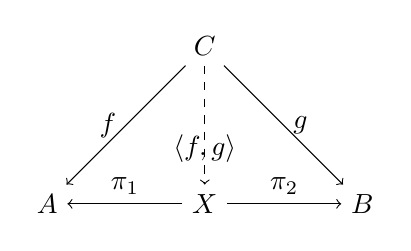
\begin{tikzpicture}
    \node (1) {$C$};
    \node[below of=1,yshift=-1cm] (2) {$X$};
    \node[left of=2,xshift=-1cm] (3) {$A$};
    \node[right of=2,xshift=1cm] (4) {$B$};

    \draw[dashed,->] (1) -- node[below] {$\langle f , g \rangle$} (2);
    \draw[->] (1) -- node[left] {$f$} (3);
    \draw[->] (1) -- node[right] {$g$} (4);
    \draw[->] (2) -- node[above] {$\pi_1$} (3);
    \draw[->] (2) -- node[above] {$\pi_2$} (4);
  \end{tikzpicture}
  \hfill{}
  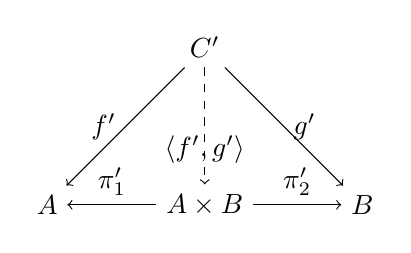
\begin{tikzpicture}
    \node (1) {$C'$};
    \node[below of=1,yshift=-1cm] (2) {$A \times B$};
    \node[left of=2,xshift=-1cm] (3) {$A$};
    \node[right of=2,xshift=1cm] (4) {$B$};

    \draw[dashed,->] (1) -- node[below] {$\langle f' , g' \rangle$} (2);
    \draw[->] (1) -- node[left] {$f'$} (3);
    \draw[->] (1) -- node[right] {$g'$} (4);
    \draw[->] (2) -- node[above] {$\pi'_1$} (3);
    \draw[->] (2) -- node[above] {$\pi'_2$} (4);
  \end{tikzpicture}
  \hfill{}

  Taking $f = \pi_1'$, $g = \pi_2'$, $f' = \pi_1$, and $g' = \pi_2$, we have an isomorphism between $X$ and $A \times B$ from the arrows $\langle f , g \rangle$ and $\langle f' , g' \rangle$.
  \begin{center}
    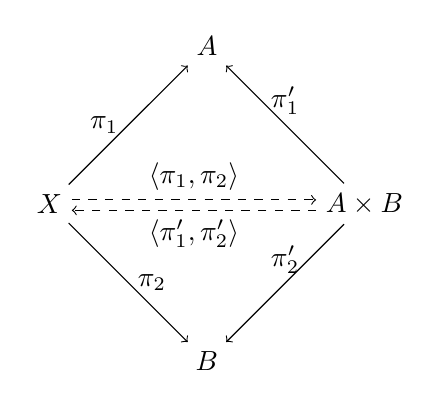
\begin{tikzpicture}
      \node (0) {};
      \node[left of=0,xshift=-1cm] (1) {$X$};
      \node[right of=0,xshift=1cm] (2) {$A \times B$};
      \node[above of=0,yshift=1cm] (3) {$A$};
      \node[below of=0,yshift=-1cm] (4) {$B$};

      \draw[transform canvas={yshift=0.3ex},dashed,->] (1) -- node[above] {$\langle \pi_1 , \pi_2 \rangle$} (2);
      \draw[transform canvas={yshift=-0.5ex},dashed,->] (2) -- node[below] {$\langle \pi'_1, \pi'_2 \rangle$} (1);
      \draw[->] (1) -- node[left] {$\pi_1$} (3);
      \draw[->] (1) -- node[right] {$\pi_2$} (4);
      \draw[->] (2) -- node[above] {$\pi'_1$} (3);
      \draw[->] (2) -- node[above] {$\pi'_2$} (4);
    \end{tikzpicture}
  \end{center}
  
  %% TODO
  For the second half of the problem, we want to show that an object $C$ isomorphic to a product object $A \times B$ is a product of $A$ and $B$.
  The isomorphism and definition of $A \times B$ give us the diagram:
  \begin{center}
    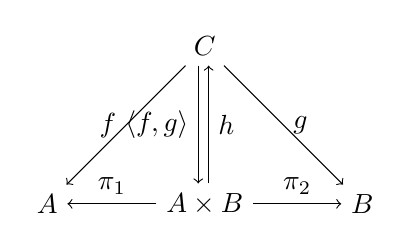
\begin{tikzpicture}
      \node (1) {$C$};
      \node[below of=1,yshift=-1cm] (2) {$A \times B$};
      \node[left of=2,xshift=-1cm] (3) {$A$};
      \node[right of=2,xshift=1cm] (4) {$B$};

      \draw[transform canvas={xshift=-0.5ex},->] (1) -- node[left] {$\langle f , g \rangle$} (2);
      \draw[transform canvas={xshift=0.3ex},->] (2) -- node[right] {$h$} (1);
      \draw[->] (1) -- node[left] {$f$} (3);
      \draw[->] (1) -- node[right] {$g$} (4);
      \draw[->] (2) -- node[above] {$\pi_1$} (3);
      \draw[->] (2) -- node[above] {$\pi_2$} (4);
    \end{tikzpicture}
  \end{center}

  From which it is clear that $h$ is $\langle \pi_1 , \pi_2 \rangle$ and $f$ and $g$ are the projections from $C$.
\newpage
\item [1.5.6.1]
  We want to show that $\langle f \circ h, g \circ h\rangle = \langle f, g \rangle \circ h$.
  The arrow $\langle f , g \rangle$ implies the existence of a product object:
  \begin{center}
    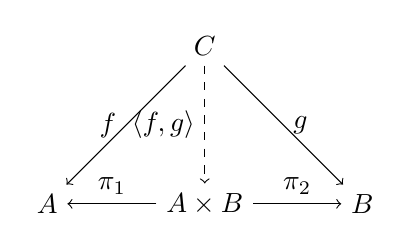
\begin{tikzpicture}
      \node (1) {$C$};
      \node[below of=1,yshift=-1cm] (2) {$A \times B$};
      \node[left of=2,xshift=-1cm] (3) {$A$};
      \node[right of=2,xshift=1cm] (4) {$B$};

      \draw[dashed,->] (1) -- node[left] {$\langle f , g \rangle$} (2);
      \draw[->] (1) -- node[left] {$f$} (3);
      \draw[->] (1) -- node[right] {$g$} (4);
      \draw[->] (2) -- node[above] {$\pi_1$} (3);
      \draw[->] (2) -- node[above] {$\pi_2$} (4);
    \end{tikzpicture}
  \end{center}

  The composition $\langle f , g \rangle \circ h$ for a function $h : D \rightarrow C$ means we have another object out in space:
  \begin{center}
    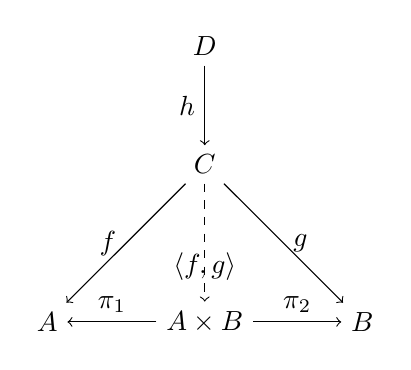
\begin{tikzpicture}
      \node (1) {$C$};
      \node[below of=1,yshift=-1cm] (2) {$A \times B$};
      \node[left of=2,xshift=-1cm] (3) {$A$};
      \node[right of=2,xshift=1cm] (4) {$B$};
      \node[above of=1,yshift=0.5cm] (5) {$D$};

      \draw[dashed,->] (1) -- node[below] {$\langle f , g \rangle$} (2);
      \draw[->] (1) -- node[left] {$f$} (3);
      \draw[->] (1) -- node[right] {$g$} (4);
      \draw[->] (2) -- node[above] {$\pi_1$} (3);
      \draw[->] (2) -- node[above] {$\pi_2$} (4);
      \draw[->] (5) -- node[left] {$h$} (1);
    \end{tikzpicture}
  \end{center}

  By composition, we obtain the arrows $f \circ h$ and $g \circ h$:
  \begin{center}
    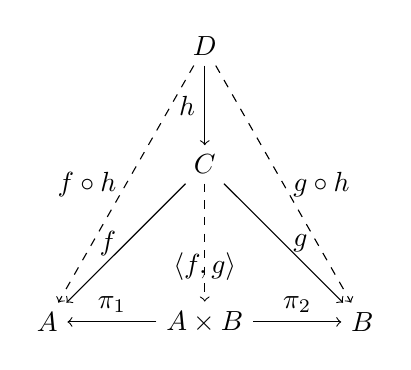
\begin{tikzpicture}
      \node (1) {$C$};
      \node[below of=1,yshift=-1cm] (2) {$A \times B$};
      \node[left of=2,xshift=-1cm] (3) {$A$};
      \node[right of=2,xshift=1cm] (4) {$B$};
      \node[above of=1,yshift=0.5cm] (5) {$D$};

      \draw[dashed,->] (1) -- node[below] {$\langle f , g \rangle$} (2);
      \draw[->] (1) -- node[left] {$f$} (3);
      \draw[->] (1) -- node[right] {$g$} (4);
      \draw[->] (2) -- node[above] {$\pi_1$} (3);
      \draw[->] (2) -- node[above] {$\pi_2$} (4);
      \draw[->] (5) -- node[left] {$h$} (1);
      \draw[dashed,->] (5) -- node[left] {$f \circ h$} (3);
      \draw[dashed,->] (5) -- node[right] {$g \circ h$} (4);
    \end{tikzpicture}
  \end{center}

  In turn, this satisfies the product construction, thus the arrows $\langle f \circ h, g \circ h \rangle$ and $\langle f , g \rangle \circ h$ are equal.
  \begin{center}
    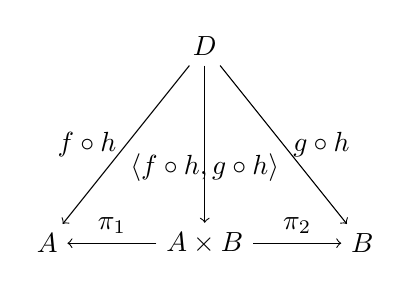
\begin{tikzpicture}
      \node (1) {};
      \node[below of=1,yshift=-0.0cm] (2) {$A \times B$};
      \node[left of=2,xshift=-1cm] (3) {$A$};
      \node[right of=2,xshift=1cm] (4) {$B$};
      \node[above of=1,yshift=0.5cm] (5) {$D$};

      %% \draw[dashed,->] (1) -- node[left] {$\langle f , g \rangle$} (2);
      %% \draw[->] (1) -- node[left] {$f$} (3);
      %% \draw[->] (1) -- node[right] {$g$} (4);
      \draw[->] (2) -- node[above] {$\pi_1$} (3);
      \draw[->] (2) -- node[above] {$\pi_2$} (4);
      \draw[->] (5) -- node[below] {$\langle f \circ h, g \circ h \rangle$} (2);
      \draw[->] (5) -- node[left] {$f \circ h$} (3);
      \draw[->] (5) -- node[right] {$g \circ h$} (4);
    \end{tikzpicture}
  \end{center}

\item [1.5.6.2]
\item [1.5.6.3]
\item [1.5.6.4]
  If $X$ and $Y$ are objects in a poset $P$ considered as a category, a product of $X$ and $Y$ is an object $Z$ such that:
  \begin{itemize}
  \item There exist arrows $\pi_1 : Z \rightarrow X$ and $\pi_2 : Z \rightarrow Y$.
  \item For every other object $C$ with arrows $f : C \rightarrow X$ and $g : C \rightarrow Y$, there is the unique arrow $\langle f , g \rangle : C \rightarrow X \times Y$.
  \end{itemize}
  In a poset considered as a category, this means that $X \times Y \le X$ and $X \times Y \le Y$.
  Additionally, we have that for all objects $C$ satisfying $C \le X \wedge C \le Y$ we have that $C \le X \times Y$.

  In other words, the product of $X$ and $Y$ is $X$ is $X \le Y$ holds and $Y$ otherwise.

\item [1.5.6.5]
  If $X$ and $Y$ are objects in a poset $P$ considered as a category, a coproduct of $X$ and $Y$ has the properties:
  \begin{itemize}
  \item $X \le X + Y$
  \item $Y \le X + Y$
  \item For every $Z$ such that $X \le Z$ and $Y \le Z$, we have $X + Y \le Z$.
  \end{itemize}

  The coproduct of $X$ and $Y$ is the greater of $X$ and $Y$.
  That is, $Y$ if $X \le Y$ and $X$ otherwise.

\item [1.5.6.6]
  The category poset has pairs of objects that lack a product (unless the poset is linear and finite).

  The discrete category has no products, nor does the category \textbf{1}.

\item [1.5.6.7]
  

\end{enumerate}
\end{document}
